%*****************************************************
%	APPENDIX
%*****************************************************
\appendix
%-----------------------------------------------------
\chapter{Standard Quadrotor Dynamics}
\label{app:stddynamics}
%-----------------------------------------------------

%-----------------------------------------------------
\chapter{Design Bill of Materials}
\label{app:bom}
%-----------------------------------------------------
\section{Parts List}
%-----------------------------------------------------
\begin{table}[htbp]
\centering
\begin{tabularx}{\textwidth}{|X|l|l|}
\hline
\multicolumn{1}{|c|}{Part Name} & Amount Used & Unit Weight[g]\\ \hline
\multicolumn{3}{|c|}{Electronics}\\ \hline
SPRacing F3 Deluxe Flight Controller & 1 & 6\\ \hline
OrangeRx 615X 2.4 GHz 6CH Receiver & 1 & 9.8\\ \hline
Signal Converter SBUS-PPM-PWM & 1 & 5.0\\ \hline 
STLink-V2 Debugger & 1 & N/A\\ \hline
RotorStar Super Mini S-BEC 10A & 1 & 30\\ \hline
128x96" OLED Display & 1 & N/A \\ \hline
XBee-Pro S1 & 2 & N/A \\ \hline
HobbyWing XRotor 15A Opto ESC & 4 & 10.5\\ \hline
OrangeRX RPM Sensor & 4 & 6\\ \hline
HobbyKing Multi-Rotor Power Distribution Board & 1 & 7.6\\ \hline
\multicolumn{3}{|c|}{Motors}\\ \hline
Corona DS-339MG & 8 & 32\\ \hline
Turnigy DST-700KV Brushlesss DC & 4 & 65\\ \hline
\multicolumn{3}{|c|}{Frame Components}\\ \hline
APM Flight Controller Damping Platform & 1 & 16\\ \hline
HobbyKing SK450 Replacement Arm (2 pcs) & 2 & N/A\\ \hline
SK450 Extended Landing Skid & 1 & 93\\ \hline
Alloy Servo Arm (FUTABA) & 8 & N/A\\ \hline
10X18X6 Radial Ball Bearing & 8 & N/A\\ \hline
80g Damping Ball & 32 & N/A\\ \hline
Plastic Retainers for Damping Balls & 32 & N/A\\ \hline
3/5mm Aluminum Prop Adapter & 4 & N/A\\ \hline
6x4.5 Gemfam 3-Blade Propeller & 4 & N/A\\ \hline
M3 6mm Hex Nylon Spacer & 8 & N/A\\ \hline
M3 16mm Hex Nylon Spacer & 32 & N/A\\ \hline
M3 25mm Nylon Screw & 128 & N/A\\ \hline
M2.5x10mm Socket Head Cap Screw & 36 & N/A\\ \hline
M2.5x25mm Socket Head Cap Screw & 20 & N/A\\ \hline
M2.5 A-Lok Nut & 16 & N/A\\ \hline 
\end{tabularx}
\label{tab:partslist}
\caption{Parts List}
\end{table}

%-----------------------------------------------------
\section{3D Printed Parts}
%-----------------------------------------------------
\begin{table}[htbp]
\centering
\begin{tabularx}{\textwidth}{|X|X|X|}
\hline
\multicolumn{3}{|c|}{Custom Printed CAD Designs}\\ \hline
\begin{minipage}{0.3\textwidth}
\centering
\hspace{8pt}
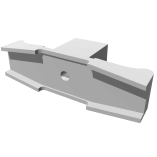
\includegraphics[width=0.95\textwidth]{figs/appendix/part_A1}
\captionof{figure}{Part A.1}
\end{minipage}
& 
\begin{minipage}{0.3\textwidth}
\centering
\hspace{8pt}
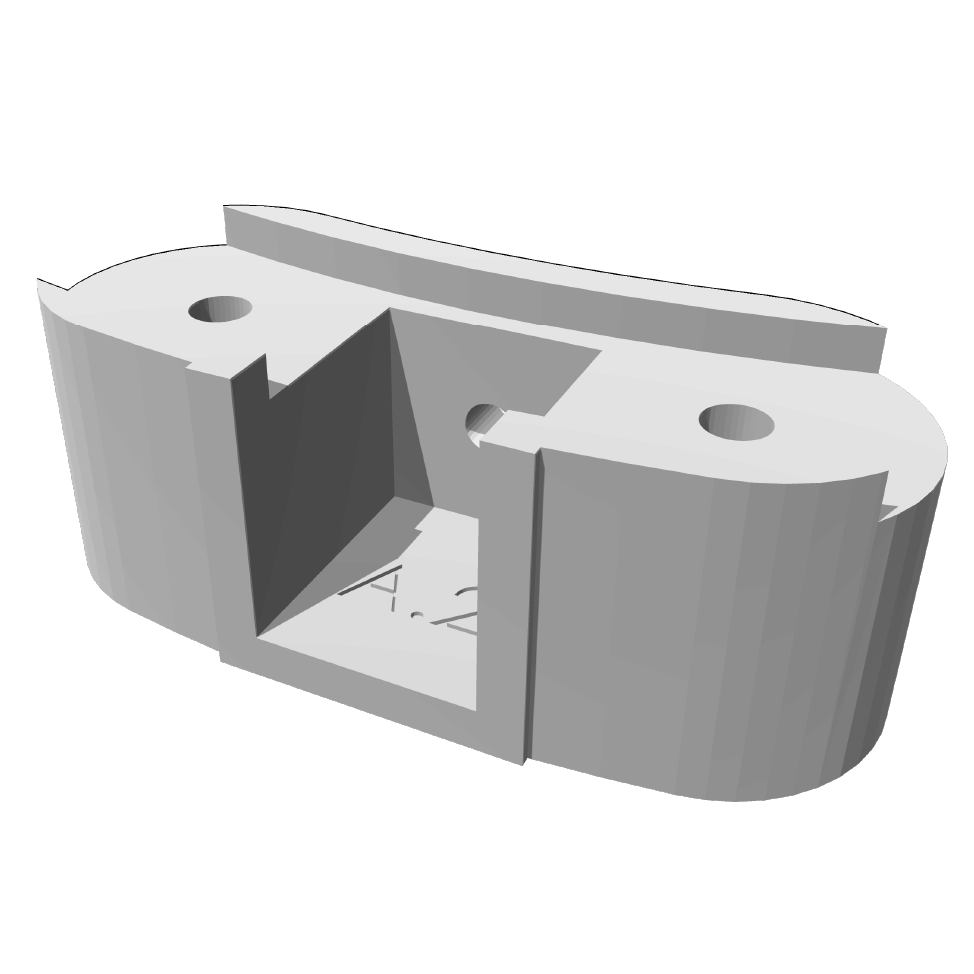
\includegraphics[width=0.95\textwidth]{figs/appendix/part_A2}
\captionof{figure}{Part A.2}
\end{minipage}
&
\begin{minipage}{0.3\textwidth}
\centering
\hspace{8pt}
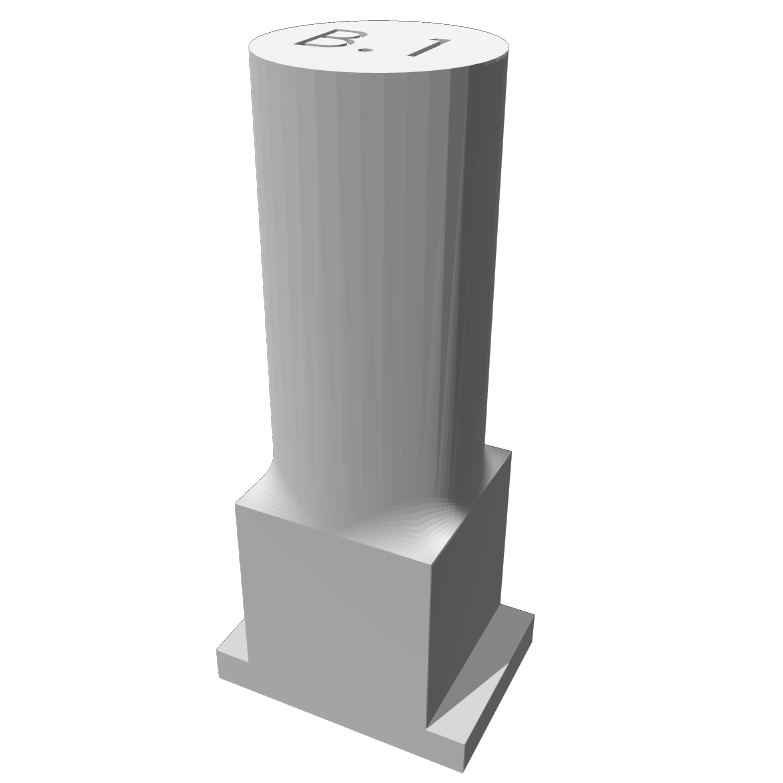
\includegraphics[width=0.95\textwidth]{figs/appendix/part_B1}
\captionof{figure}{Part B.1}
\end{minipage}
\\ \hline
\begin{minipage}{0.3\textwidth}
\centering
\hspace{8pt}
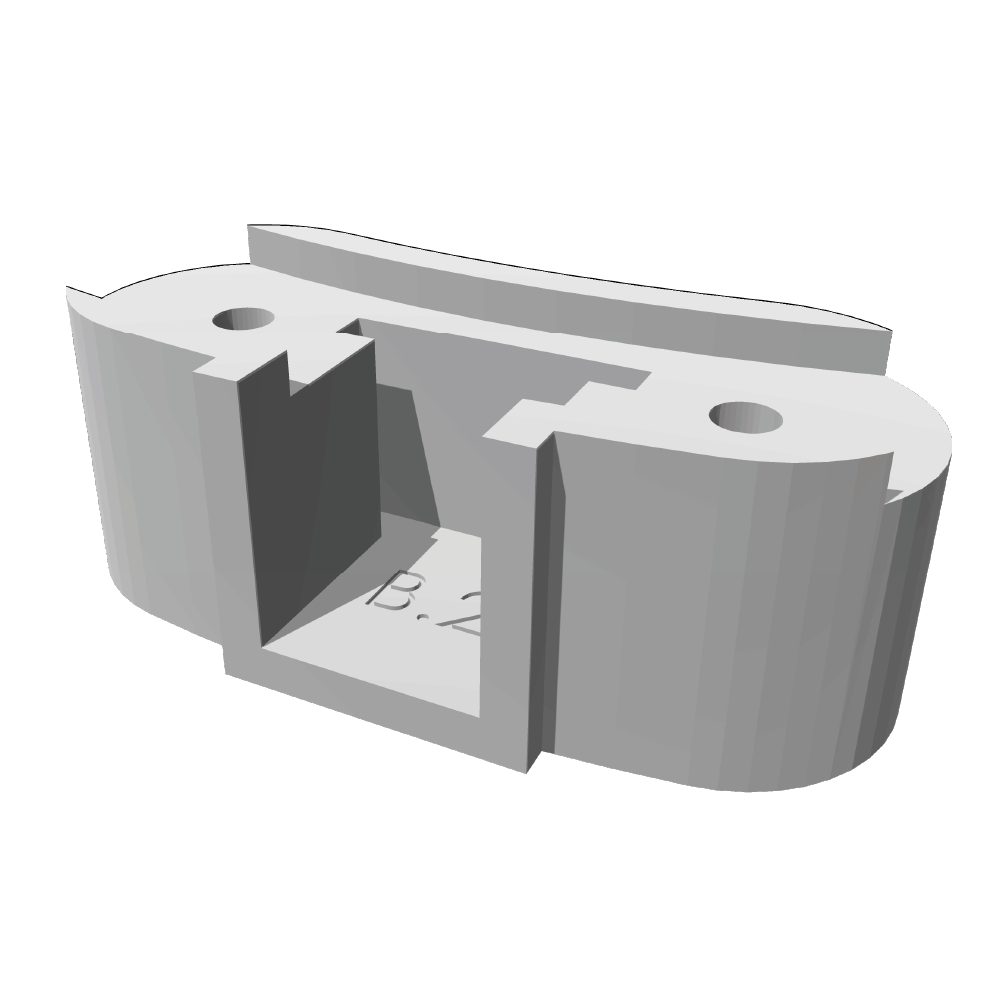
\includegraphics[width=0.95\textwidth]{figs/appendix/part_B2}
\captionof{figure}{Part B.2}
\end{minipage}
& 
\begin{minipage}{0.3\textwidth}
\centering
\hspace{8pt}
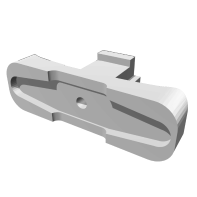
\includegraphics[width=0.95\textwidth]{figs/appendix/part_C1}
\captionof{figure}{Part C.1}
\end{minipage}
&
\begin{minipage}{0.3\textwidth}
\centering
\hspace{8pt}
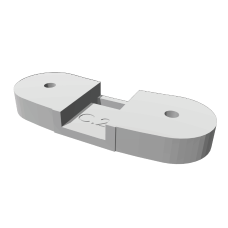
\includegraphics[width=0.95\textwidth]{figs/appendix/part_C2}
\captionof{figure}{Part C.2}
\end{minipage}
\\ \hline
\begin{minipage}{0.3\textwidth}
\centering
\hspace{8pt}
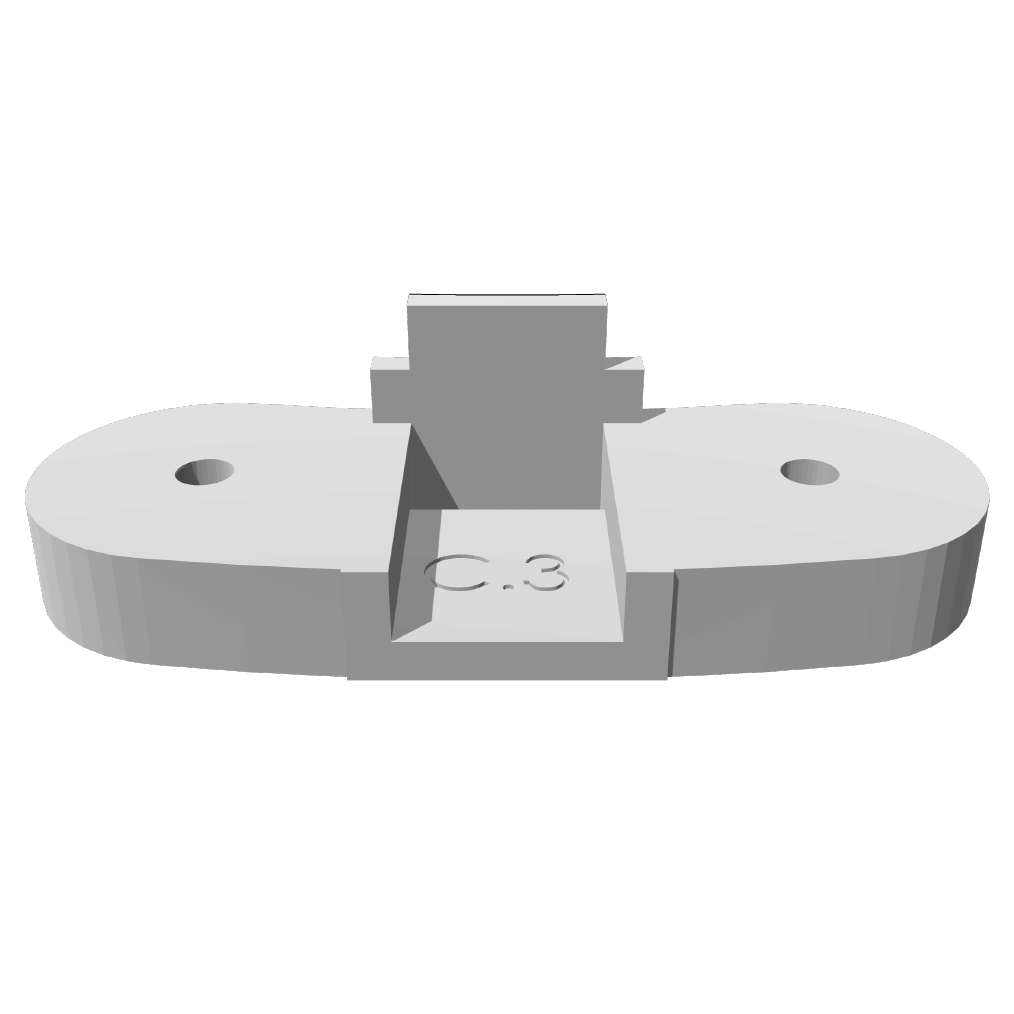
\includegraphics[width=0.95\textwidth]{figs/appendix/part_C3}
\captionof{figure}{Part C.3}
\end{minipage}
& 
\begin{minipage}{0.3\textwidth}
\centering
\hspace{8pt}
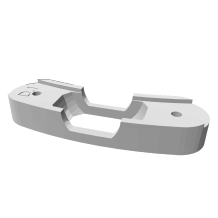
\includegraphics[width=0.95\textwidth]{figs/appendix/part_D1}
\captionof{figure}{Part D.1}
\end{minipage}
&
\begin{minipage}{0.3\textwidth}
\centering
\hspace{8pt}
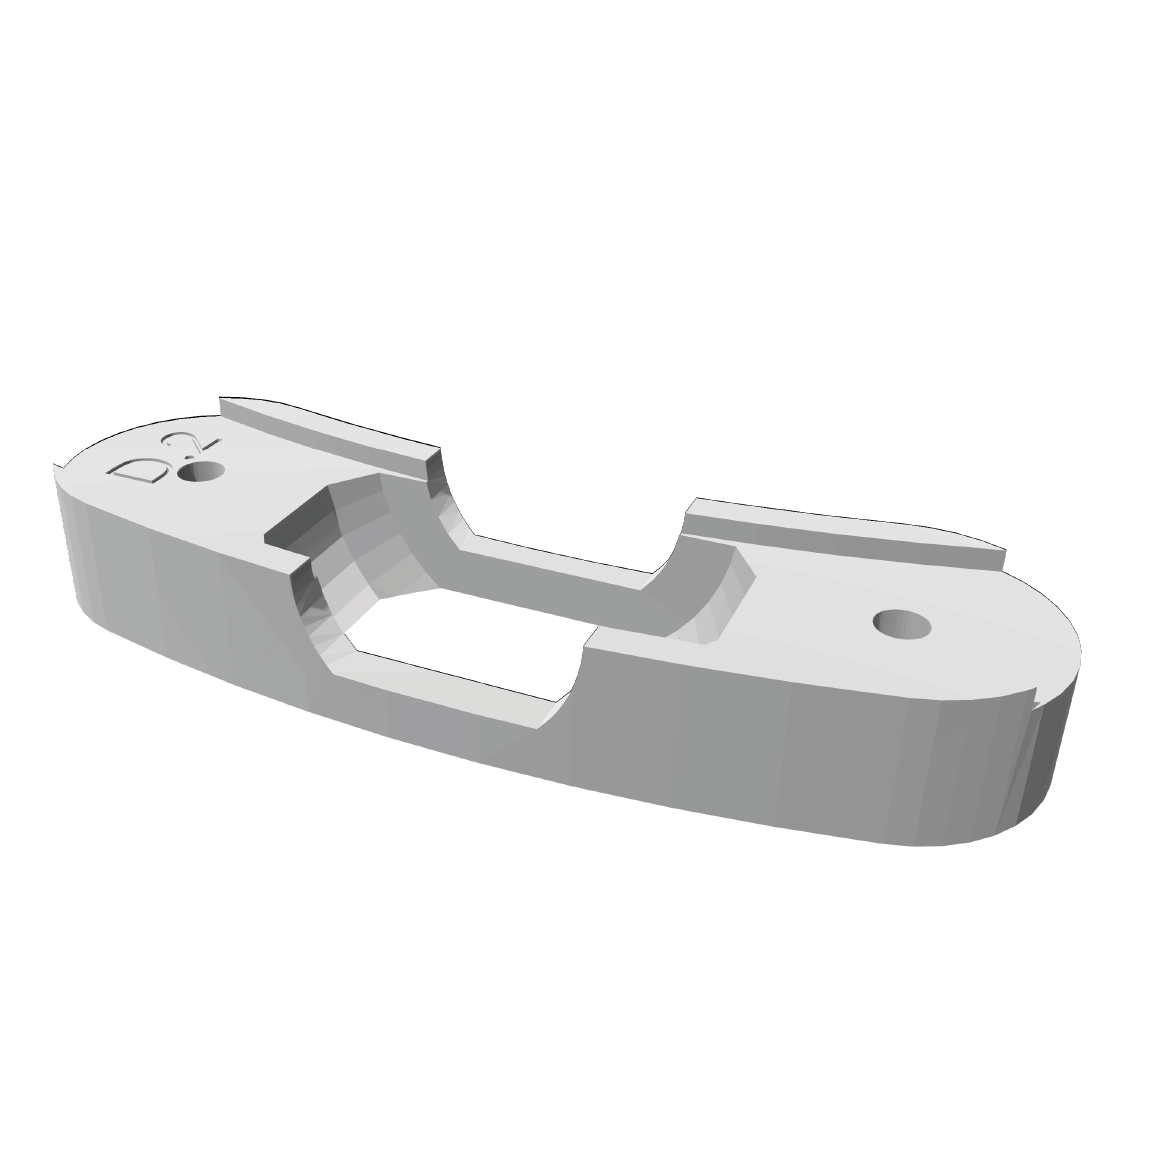
\includegraphics[width=0.95\textwidth]{figs/appendix/part_D2}
\captionof{figure}{Part D.2}
\end{minipage}
\\ \hline
\begin{minipage}{0.3\textwidth}
\centering
\hspace{8pt}
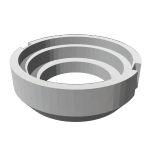
\includegraphics[width=0.95\textwidth]{figs/appendix/part_D3}
\captionof{figure}{Part D.3}
\end{minipage}
& 
\begin{minipage}{0.3\textwidth}
\centering
\hspace{8pt}
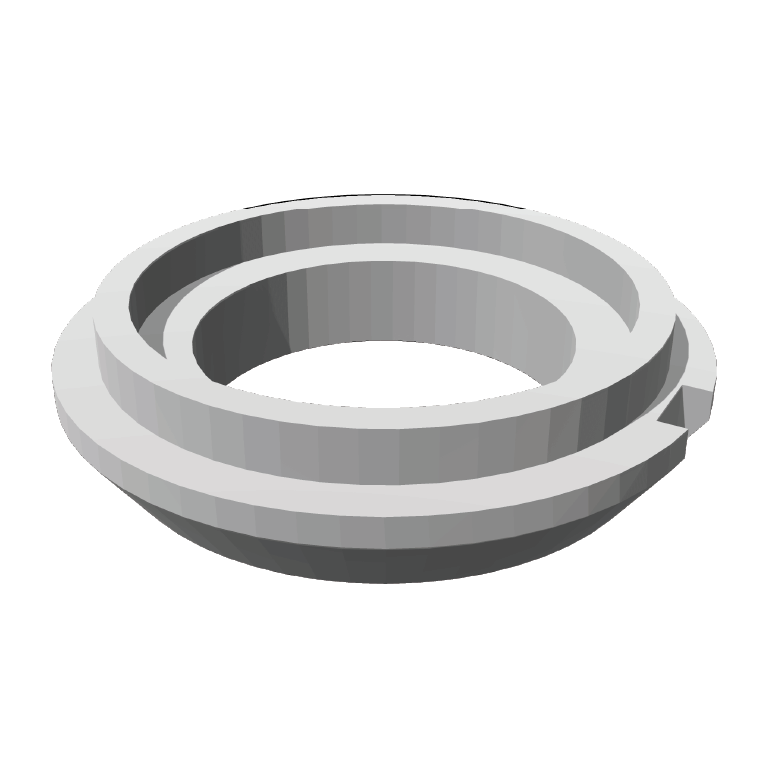
\includegraphics[width=0.95\textwidth]{figs/appendix/part_D4}
\captionof{figure}{Part D.4}
\end{minipage}
&
\begin{minipage}{0.3\textwidth}
\centering
\hspace{8pt}
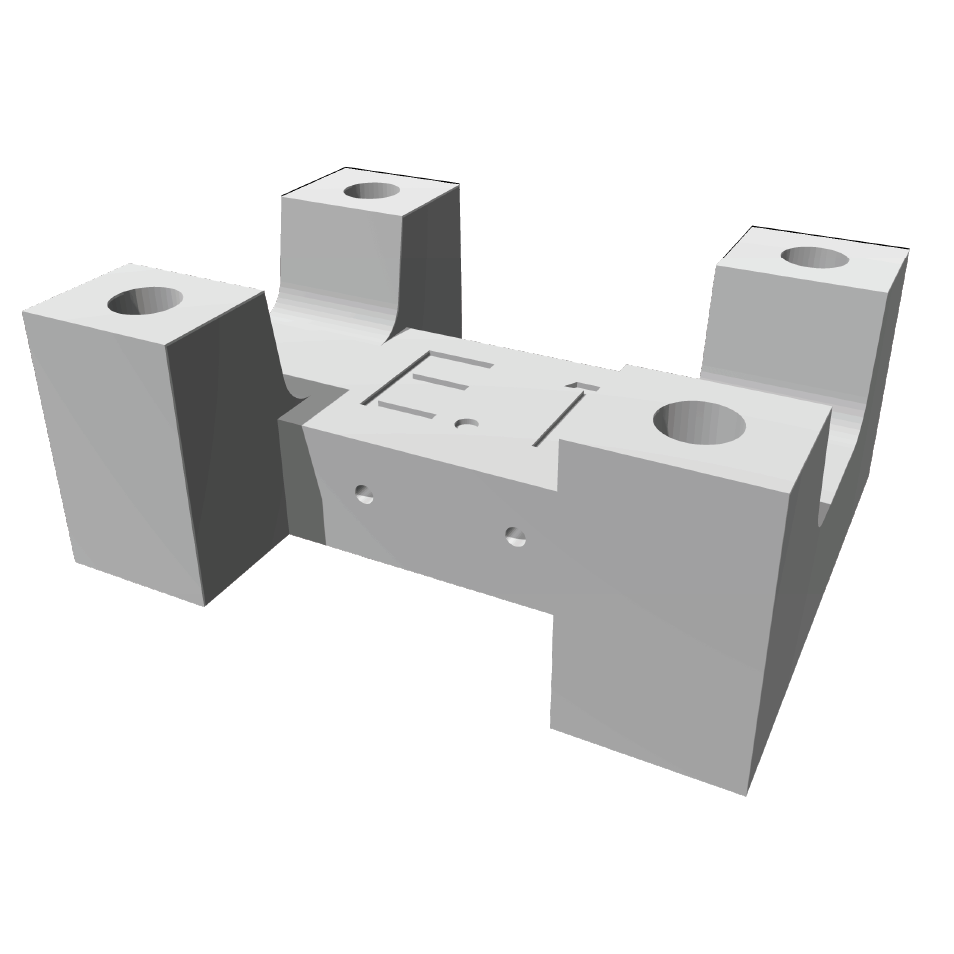
\includegraphics[width=0.95\textwidth]{figs/appendix/part_E1}
\captionof{figure}{Part E.1}
\end{minipage}
\\ \hline
\end{tabularx}
\end{table}
\newpage
%-----------------------------------------------------
%Table 2
%-----------------------------------------------------
\begin{table}[hbtp]
\centering
\begin{tabularx}{\textwidth}{|X|X|X|}
\hline
\begin{minipage}{0.3\textwidth}
\centering
\hspace{10pt}
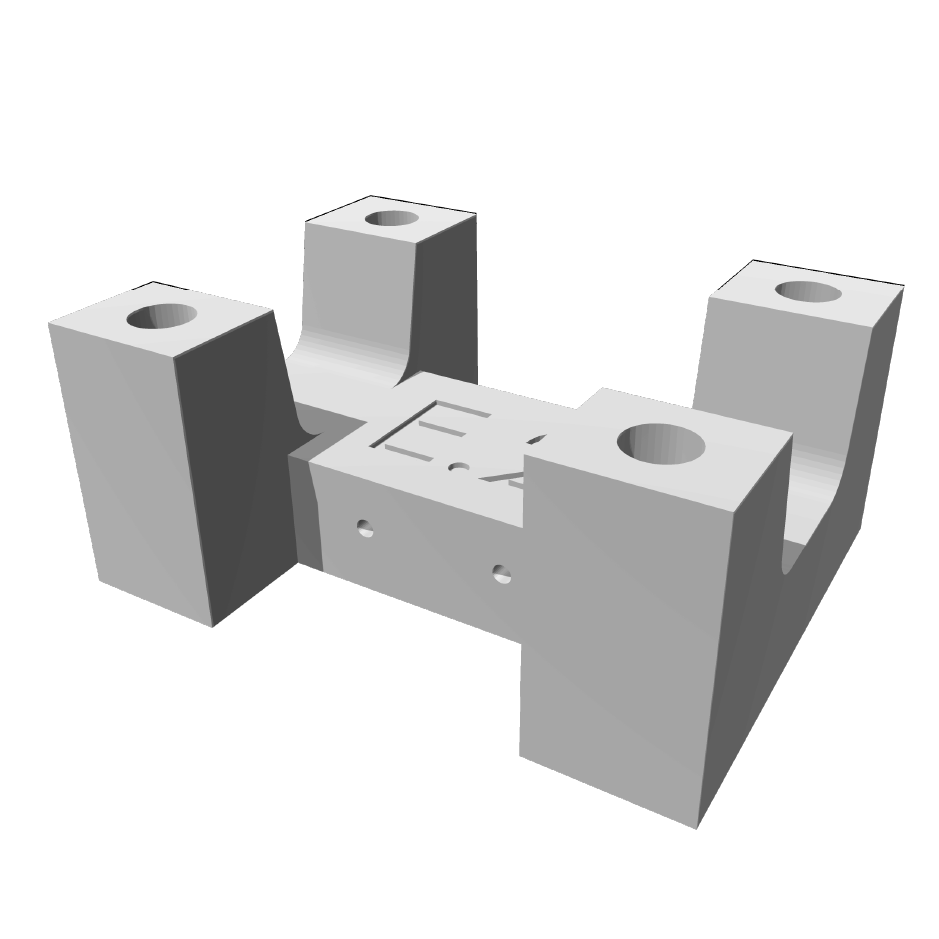
\includegraphics[width=0.95\textwidth]{figs/appendix/part_E2}
\captionof{figure}{Part E.2}
\end{minipage}
& 
\begin{minipage}{0.3\textwidth}
\centering
\hspace{10pt}
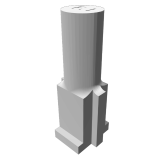
\includegraphics[width=0.95\textwidth]{figs/appendix/part_F1}
\captionof{figure}{Part F.1}
\end{minipage}
&
\begin{minipage}{0.3\textwidth}
\centering
\hspace{10pt}
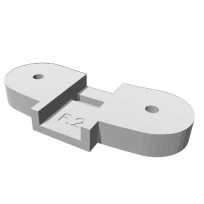
\includegraphics[width=0.95\textwidth]{figs/appendix/part_F2}
\captionof{figure}{Part F.2}
\end{minipage}
\\ \hline
\begin{minipage}{0.3\textwidth}
\centering
\hspace{10pt}
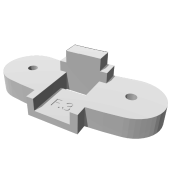
\includegraphics[width=0.95\textwidth]{figs/appendix/part_F3}
\captionof{figure}{Part F.3}
\end{minipage}
& 
\begin{minipage}{0.3\textwidth}
\centering
\hspace{10pt}
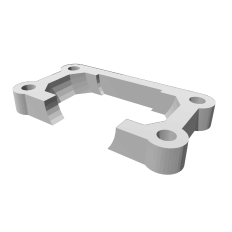
\includegraphics[width=0.95\textwidth]{figs/appendix/part_G1}
\captionof{figure}{Part G.1}
\end{minipage}
&
\begin{minipage}{0.3\textwidth}
\centering
\hspace{10pt}
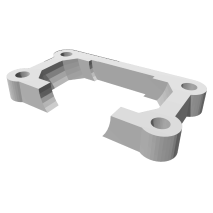
\includegraphics[width=0.95\textwidth]{figs/appendix/part_G2}
\captionof{figure}{Part G.2}
\end{minipage}
\\ \hline
\begin{minipage}{0.3\textwidth}
\centering
\hspace{10pt}
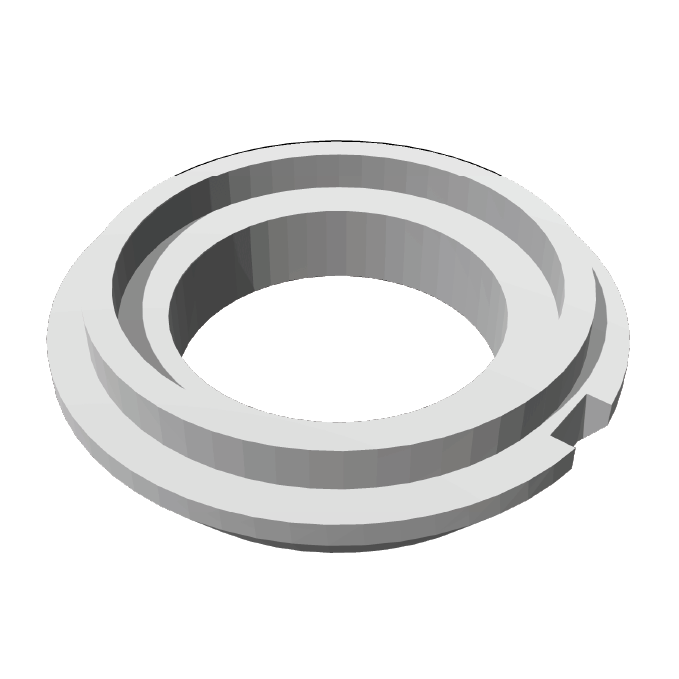
\includegraphics[width=0.95\textwidth]{figs/appendix/part_G3}
\captionof{figure}{Part G.3}
\end{minipage}
& 
\begin{minipage}{0.3\textwidth}
\centering
\hspace{10pt}
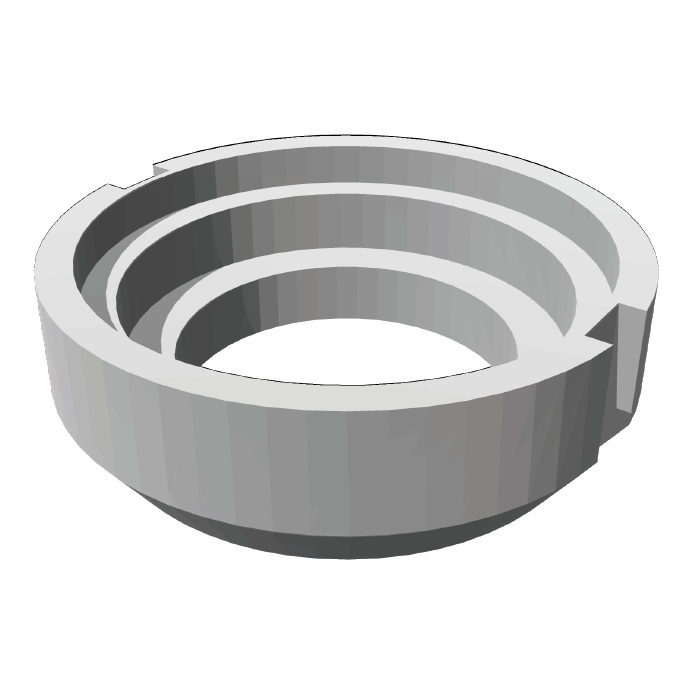
\includegraphics[width=0.95\textwidth]{figs/appendix/part_G4}
\captionof{figure}{Part G.4}
\end{minipage}
&
\begin{minipage}{0.3\textwidth}
\centering
\hspace{10pt}
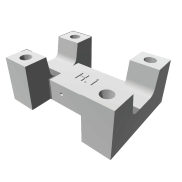
\includegraphics[width=0.95\textwidth]{figs/appendix/part_H1}
\captionof{figure}{Part H.1}
\end{minipage}
\\ \hline
\begin{minipage}{0.3\textwidth}
\centering
\hspace{10pt}
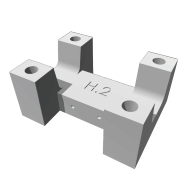
\includegraphics[width=0.95\textwidth]{figs/appendix/part_H2}
\captionof{figure}{Part H.2}
\end{minipage}
\\
%\cline{1-2}
\end{tabularx}
\end{table}
%-----------------------------------------------------
\section{Lasercut Components}
%-----------------------------------------------------
\section{Assembly}
%-----------------------------------------------------
%-----------------------------------------------------
\chapter{System ID Test Data}
\label{app:systemdat}
%-----------------------------------------------------
\chapter{Full Equations}
\label{app:eq}
\section{Inertias}
\begin{subequations}
\begin{equation} \label{eq:app.inertia}
\approx\begin{bmatrix}
3613.144 & 0.025 & 406.81\\
0.025 & 9774.160 & 0.4626\\
406.81 & 0.4626 & 12650.72\\
\end{bmatrix}
\end{equation}
\vspace{-5pt}
\begin{equation}
\begin{bmatrix}
0 & -0.249s\lambda-0.276c\lambda & 0.249c\lambda-0.276s\lambda\\
-0.249s\lambda-0.276c\lambda & -0.448s2\lambda -2142.67s\lambda+983c\lambda&983s2\lambda-2142.67s\lambda+0.448c2\lambda\\
0.249c\lambda-0.276s\lambda & 983s2\lambda -2142.67s\lambda +0.448c2\lambda & 1967.497s\lambda + 1070.88c2\lambda+0.448s2\lambda\\
\end{bmatrix}
\end{equation}
\end{subequations}